\section{Introduction}
\label{sec:introduction}

\begin{figure}[htb] \centering
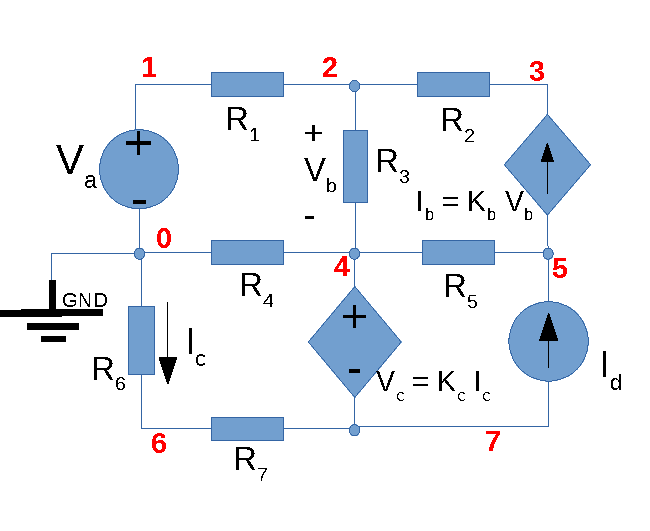
\includegraphics[width=0.4\linewidth]{rcm.pdf}
\caption{Nodal representation of the circuit.}
\label{fig:rc}
\end{figure}

\begin{table}[H]
  \centering
  \begin{tabular}{|l|r|}
    \hline    
    {\bf Name} & {\bf Value} \\ \hline
    R(1) & 1.015259 \\  \hline 
R(2) & 2.090689 \\  \hline 
R(3) & 3.108356 \\  \hline 
R(4) & 4.101243 \\  \hline 
R(5) & 3.033480 \\  \hline 
R(6) & 2.009605 \\  \hline 
R(7) & 1.005573 \\  \hline 
C & 1.015319 \\  \hlineVs & 5.026261 \\  \hlineKb & 7.161103 \\  \hlineKd & 8.185741 \\  \hline
  \end{tabular}
  \caption{Constants provided by Python. A variable  preceded by !! is of type {\it capacitance}
    and expressed in Farad ;a variable preceded by § is of type {\it resistence} and expressed in
    Ohm;a variable preceded by £ is of type {\it conductance} and expressed in
    Siemens; other variables are of type {\it voltage} and expressed in
    Volt.}
  \label{tab:op}
\end{table}

% state the learning objective 
The objective of this laboratory assignment is to chose the architecture of the envelope detector and voltage regulator. By doing this we will design a AC/DC converter and bear in mind that cost is a very important factor and we should make the circuit as budget friendly as possible while keeping a good or great efficiency. The circuit can be seen in Figure ~\ref{fig:rc}. 



In section 2, a theoretical analysis of the circuit is presented. In section 5, the circuit's simulation analysis results are expressed in graphics and commented. Finally, in section 6, we will compare the simulation and theoretical values and in this way conclude our study.


